\documentclass[12pt, a4paper]{article}

\usepackage{a4wide}
\usepackage{color}
\usepackage{amsmath,amssymb,epsfig,pstricks,xspace}
\usepackage{subfigure}
%\usepackage{german,graphics}
\usepackage{dsfont}
\usepackage{amsfonts}
\usepackage{graphics, psfrag}
\usepackage[latin1]{inputenc}
\usepackage[T1]{fontenc}

\usepackage{enumitem} 
\usepackage{url}
\urlstyle{same}
\usepackage{array,dcolumn,booktabs}
\usepackage{pdflscape}
\usepackage{amsthm}
\usepackage{natbib}
\usepackage{hyperref}
\hypersetup{
	colorlinks,
	citecolor=black,
	filecolor=black,
	linkcolor=black,
	urlcolor=black
}

\newbox{\bigpicturebox}
\renewcommand\harvardurl[1]{URL: \textit{#1}}

\newcounter{task}
\newcommand{\task}{\stepcounter{task}\paragraph{Task \thetask~--~
Solution}}

\usepackage{pifont}

\newcommand{\header}{
  \begin{center}
  \fbox{\parbox{12cm}{
    \begin{center}
      {\Large 08336 Neural, Emergent and\\ Agent Technology\\ \vspace{0.2em}
        {\bf ACW Part I + II}\\ \vspace{0.35em} (Spring Term 2018)\\
        \vspace{0.2em} \firstname \lastname \\      
    }
    \end{center}
  }}
  \end{center}
}


%-------------------------------------------------------------------------------
%---------------------------- EDIT FROM HERE -----------------------------------
%-------------------------------------------------------------------------------

\newcommand{\firstname}{Ephraim}
\newcommand{\lastname}{ Schott}


\begin{document}
\pagestyle{plain}
\header


% number of tasks are automatically generated
\section*{ACW Part I}
% number of tasks are automatically generated
\subsection*{Neuron model and learning setup}

In order to examine and answer the questions of this report a neuron model similar to the illustration in figure \ref{fig:neuron-model} has been implemented using python. The code can be seen in the attached file \texttt{neural\_acw\_part1.py}. The input weights were initialized with random values between 0 and 1.\\\\
\begin{figure}[htbp]
	\begin{center}
		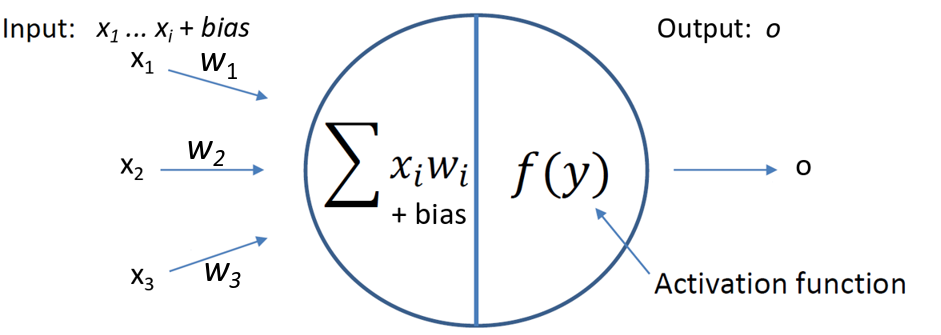
\includegraphics[width=12cm]{my_images/acw_p1/task1_neuron_model.png}
	\end{center}
	\caption{Model of a neuron or perceptron.}
	\label{fig:neuron-model}
\end{figure}\\\\
The general calculation of the output of a neuron always followed the equations $y = \sum x_iw_i + bias$ and $o = f(y)$. The weight update gets calculated by this equation $w_i = w_i * learn\_rate * (t - o) * x_i$, where $t$ is our target value. For modelling the perceptrons activation function $f(y)$ the Heaviside step function (see figure \ref{fig:activation-functions}) was used. The neuron uses the logistic sigmoid function ($\frac{1}{1 + e^{-y}} $) as $f(y)$.

\begin{figure}[htbp]
	\begin{center}
		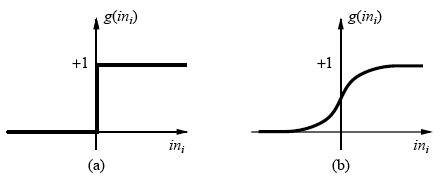
\includegraphics[width=12cm]{my_images/acw_p1/sigmoid_step_functions.png}
	\end{center}
	\caption{Used activation functions (left: step function, right: logistic sigmoid function).}
	\label{fig:activation-functions}
\end{figure}

\subsection*{Training perceptrons and neurons}

As the simple perceptron uses the Heaviside step function it is only able to create binary outputs. Figure \ref{fig:perceptron-bfr-aftr} shows that the output of the perceptron is not effected by learning. Indeed the weights of the perceptron get adjusted by each training iteration, but the adjustments can't effect or improve the binary output of the perceptron. A step function is not suitable for this task, because the task requires continuous outputs between 0 and 1 in order to make precise and useful predictions.
\begin{figure}[htbp]
	\begin{center}
		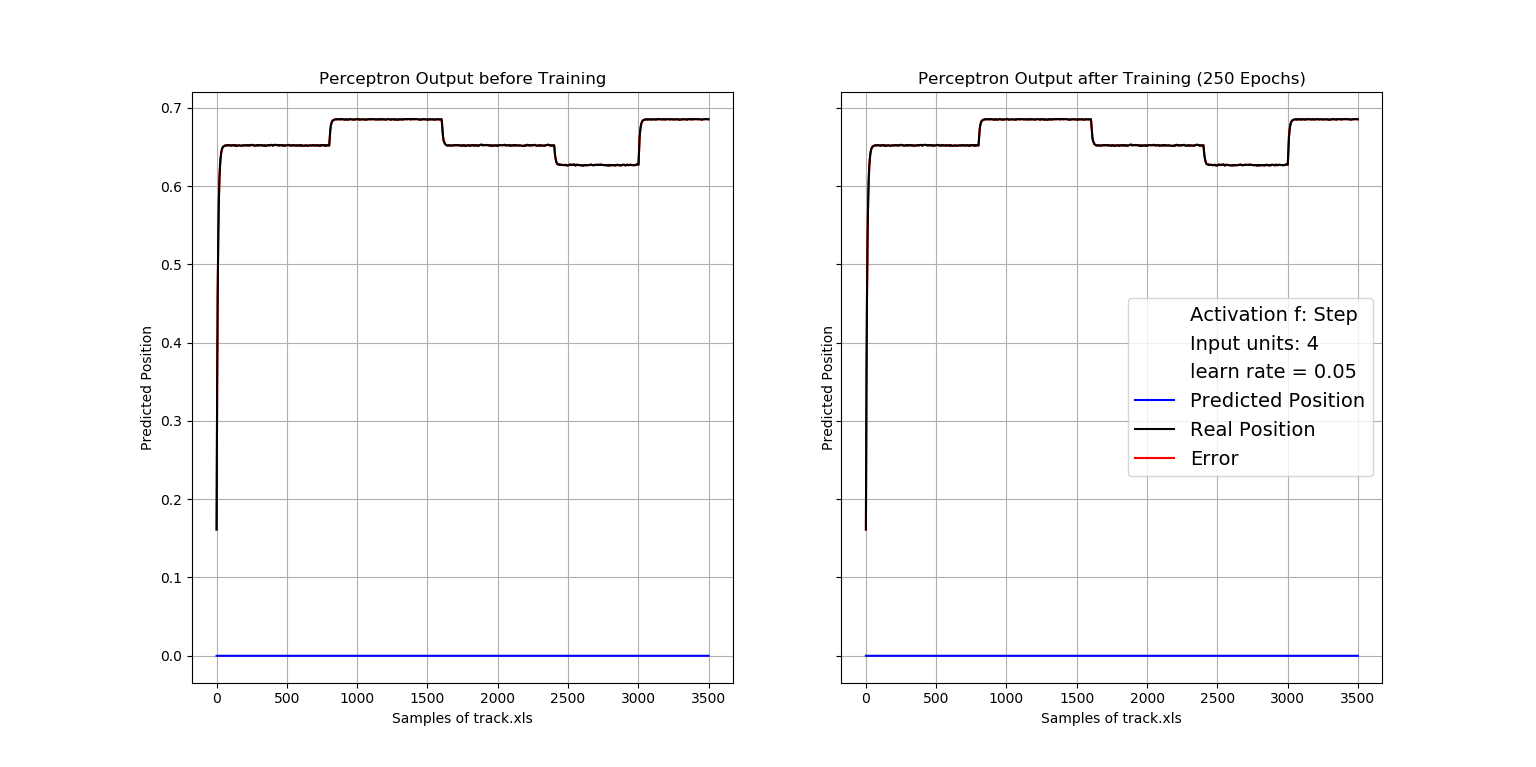
\includegraphics[width=16cm]{my_images/acw_p1/task2_perceptron_bfr_aftr.png}
	\end{center}
	\caption{Output of a perceptron with a step function before and after learning.}
	\label{fig:perceptron-bfr-aftr}
\end{figure}\\\\
The prediction results change when we replace the perceptron by a neuron which utilizes the logistic sigmoid as an activation function. The graphs of figure \ref{fig:neuron-bfr-aftr} show that the trained neuron is able to predict positions with a small error. The neuron is able to output continuous numbers that depend on, and vary according to the inputs. Through the continuous output we can obtain different delta errors in each iteration, through which we can update the weights. As one can see in figure \ref*{fig:neuron-learn} the average error of the neuron is decreasing through the training, which indicates that the neuron is now capable of learning.
\begin{figure}[htbp]
	\subfigure[The neurons average error is decreasing over all samples.]{\label{fig:neuron-learn}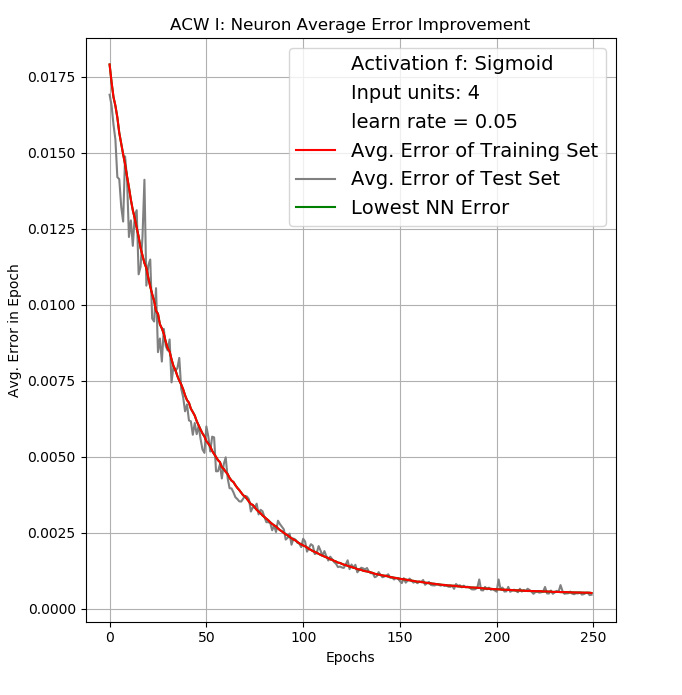
\includegraphics[width=0.45\textwidth]{my_images/acw_p1/task3_neuron_learn.png}}
	\subfigure[The predicted position of the neuron is close to the real position of the sample data after training. ]{\label{fig:neuron-bfr-aftr}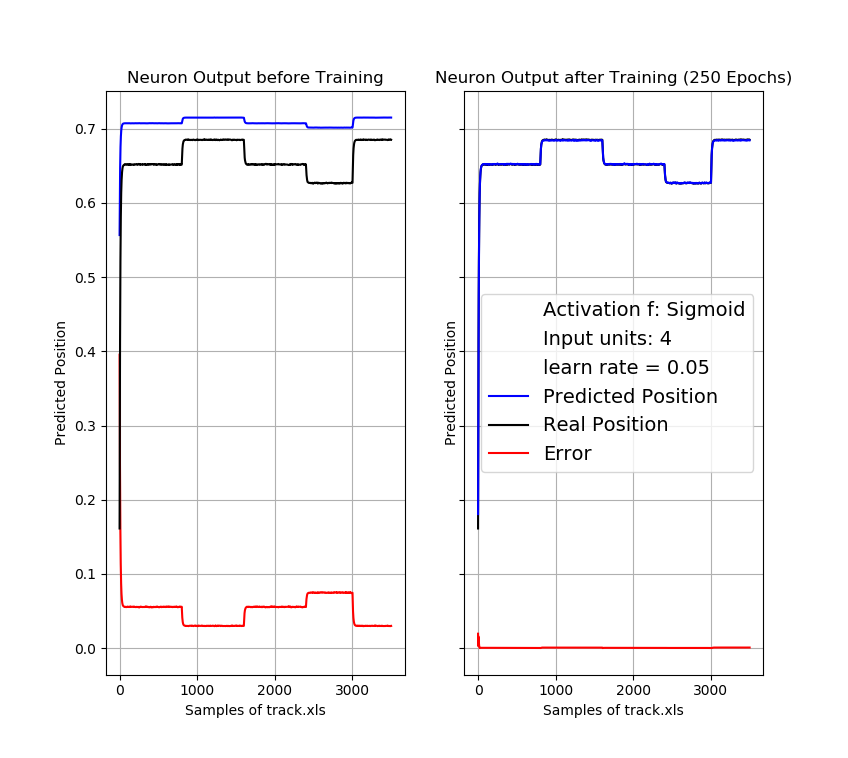
\includegraphics[width=0.549\textwidth]{my_images/acw_p1/task3_neuron_bfr_aftr.png}}
	\caption{Learning curve and outputs of a neuron with a sigmoid activation function.}
	\label{fig:neuron}
\end{figure}\\\\
In general the predictions of a neuron for a training set become more accurate the longer one trains it with the same set. In the beginning of this training the neuron will also improve its predictions for data related to the training set. With each training epoch the weights will become better in predicting particular data while their ability to generalise will decrease. By partitioning our data into trainings and test sets we can validate how good the fit of our model is and if it is \textit{over}- or \textit{underfitting} our data. When creating different data sets it is important to add some form of randomization. Figure \ref{fig:cross-validation} shows the cross validation output of a neuron which got trained with the first 2000 samples and one that got trained with shuffled data.

\begin{figure}[htbp]
	\subfigure[Trainings set not shuffled]{\label{fig:no-shuffle}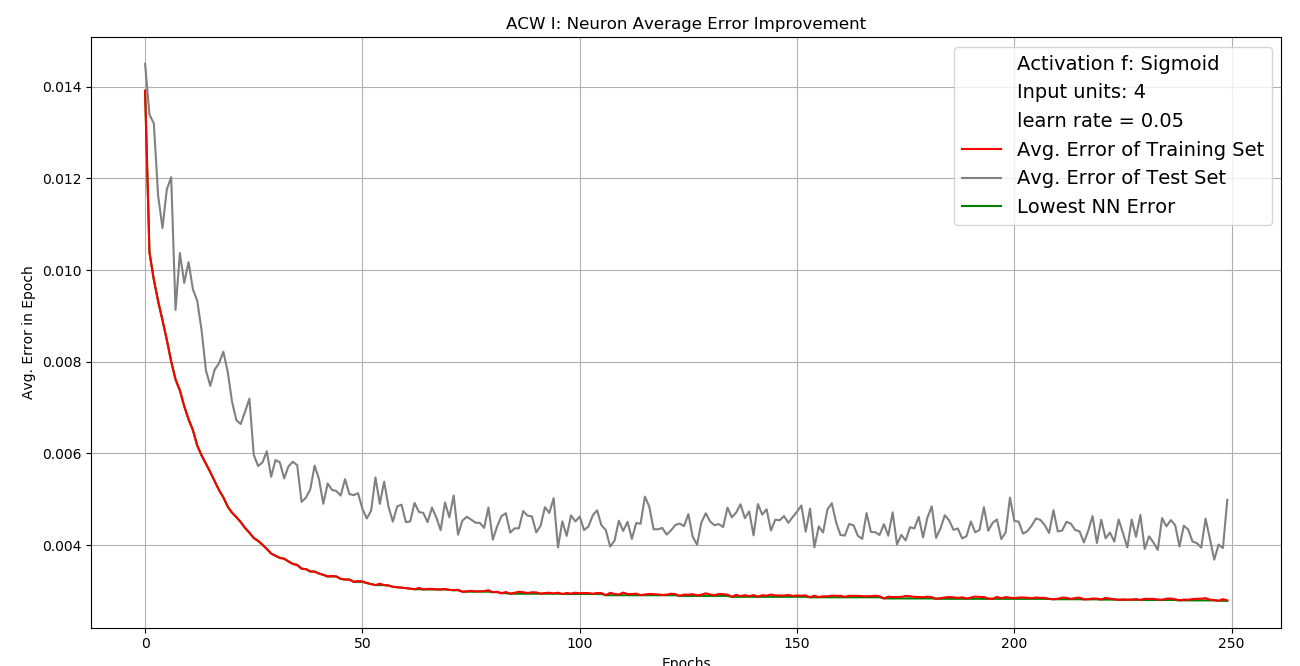
\includegraphics[width=0.5\textwidth]{my_images/acw_p1/task4_cross_learn_curve_without_shuffle.png}}
	\subfigure[Shuffled trainings set]{\label{fig:with-shuffle}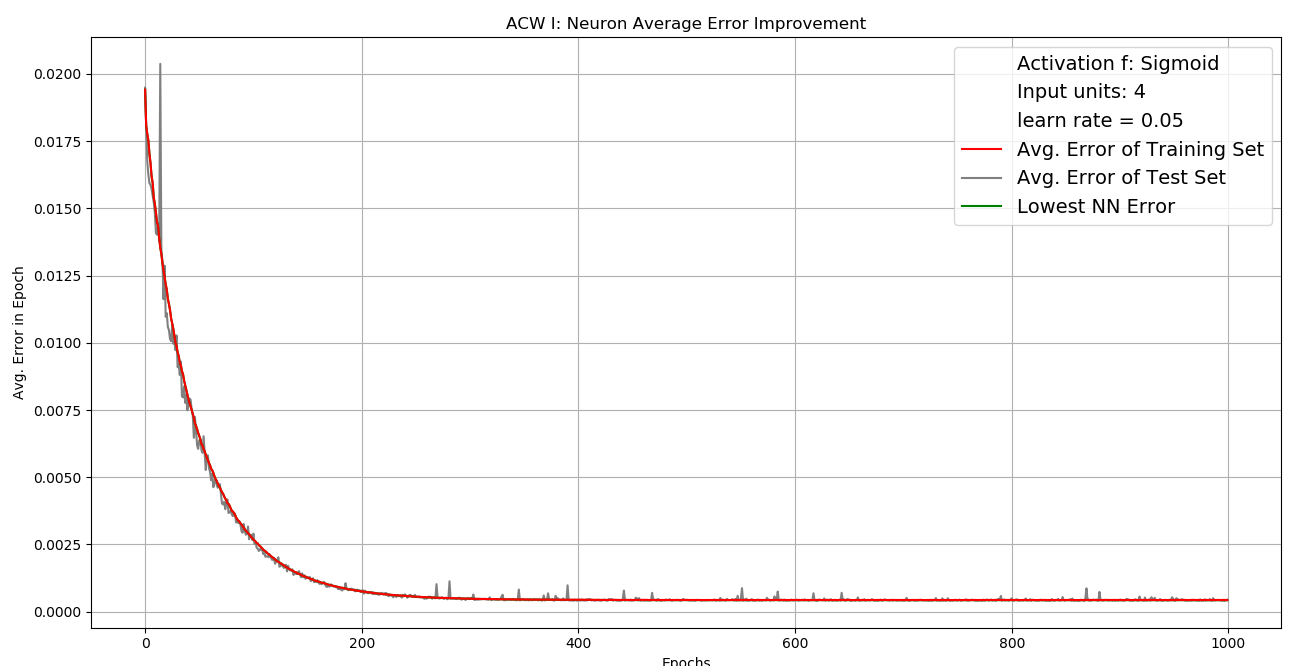
\includegraphics[width=0.5\textwidth]{my_images/acw_p1/task4_cross_learn.png}}
	\caption{Effect of shuffling the data set before cross validation learning.}
	\label{fig:cross-validation}
\end{figure}

\subsection*{Adapting the neuron to data and velocity}
The system that the neuron is predicting seems to switch between three different states. Depending on the number of inputs and the training one can observe that the predictions of the neuron are some samples behind the real output. The reason might be that the neuron realises the state transition of the system only step by step.\\\\
In order to additionally predict the velocity one need another neuron for the extra output. As the velocity depends on the position it could be useful to give the position output as an input to the velocity neuron. A multi-layered network should be helpful in this case, as it could model the dependency of position and velocity.

\section*{ACW Part II}

For the second part of this report a neural network with back propagation has been implemented using python. The code can be seen in the attached file \texttt{neural\_acw\_part2.py}. The input weights were initialized with normal distributed random values between~0~and~1.

\subsection*{Varying the number of hidden units and layers}

Changing the number of neurons has an impact on the time needed for training the network, on the improvement through learning and on the probability of learning at all. Figure \ref{fig:average-vary-units} shows that in general networks with more hidden units are learning better than networks with less hidden units. In average the networks with 30~hidden units decreased their error by around 0.23 over 250~epochs while the networks with 3~units only decreased their average error by around 0.02. Although it takes a lot longer to train networks with more nodes,
\begin{figure}[htbp]
	\subfigure[Averaged outputs of 5~NN with 3~hidden units.]{\label{fig:3-units}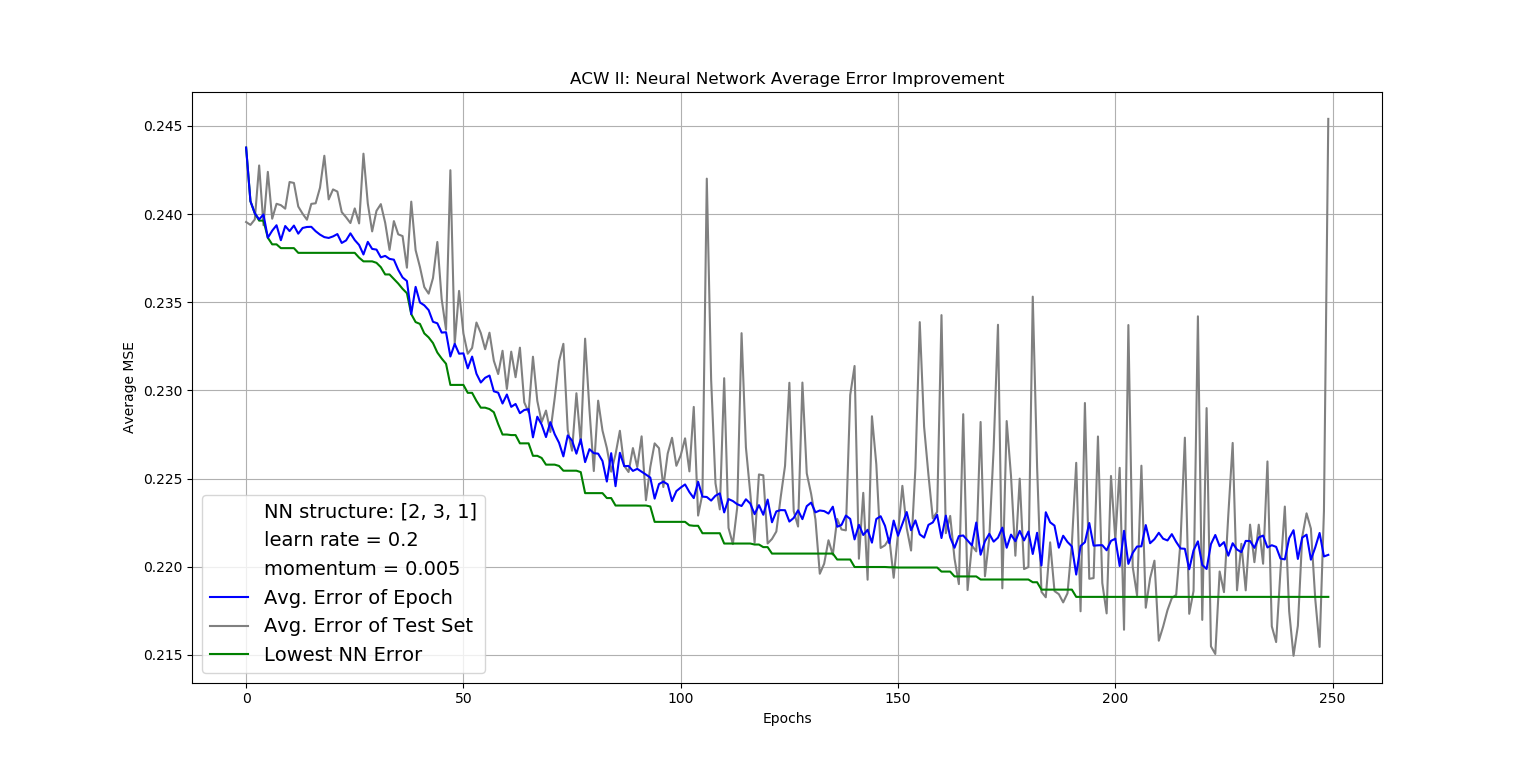
\includegraphics[width=0.5\textwidth]{my_images/acw_p2/vary_nodes_layers/improve_avg_2_3_1.png}}
	\subfigure[Averaged outputs of 5~NN with 30~hidden units]{\label{fig:30-units}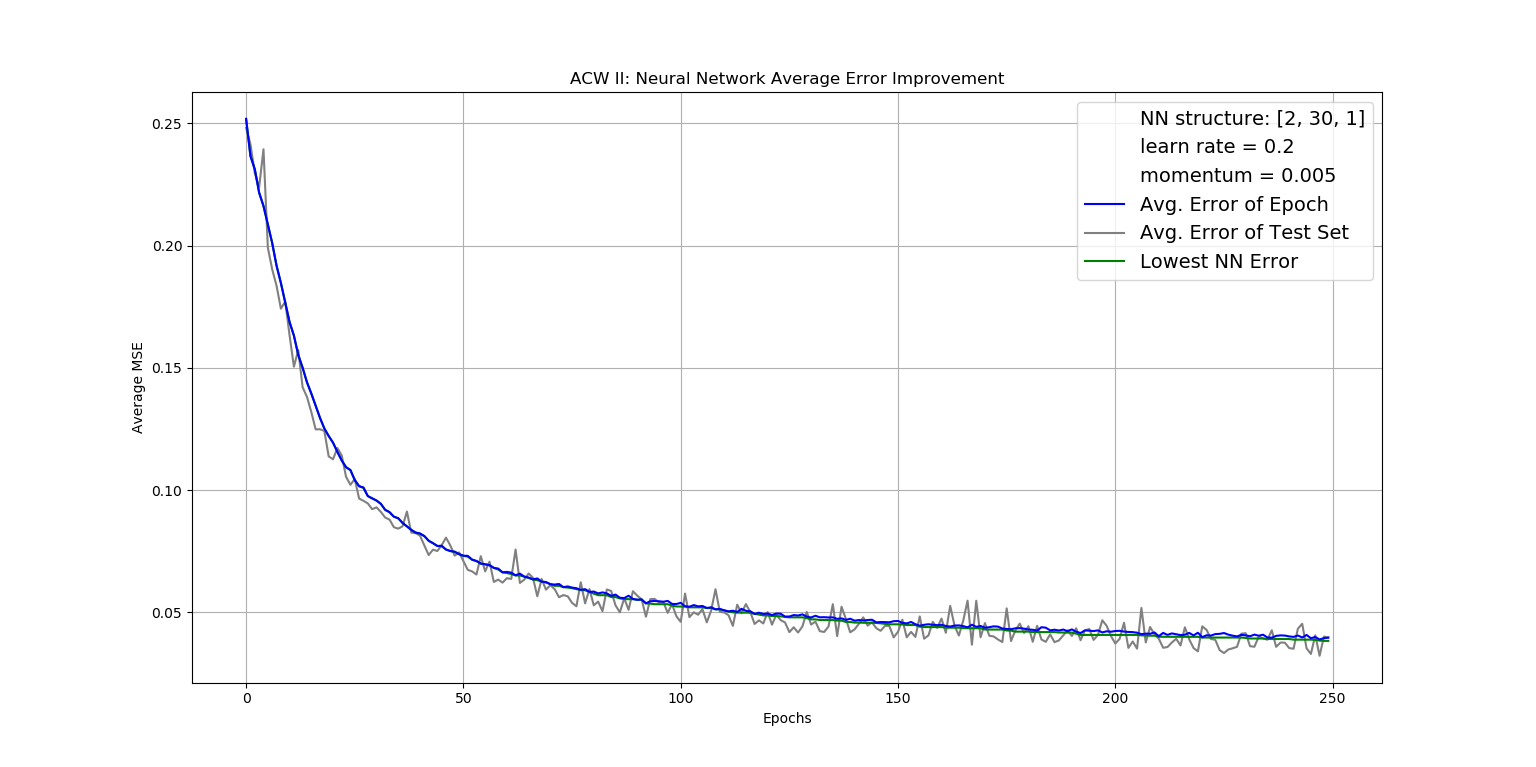
\includegraphics[width=0.5\textwidth]{my_images/acw_p2/vary_nodes_layers/improve_avg_2_30_1.png}}
	\caption{Averaged error improvement of networks with different hidden units.}
	\label{fig:average-vary-units}
\end{figure}



\subsection*{Varying the learning rate}

discussion of the results as the rate of learning is varied

discussion on the effect of a momentum term

the nature of the error as you vary the number of hidden nodes

discussion and Analysis (e.g Compare the performance of the best and worst networks)

Suggestions for further improving performance (e.g use RBFs and sample result)

\begin{figure}[htbp]
	\begin{tabular}{@{}cc@{}}
		\raisebox{-\height}{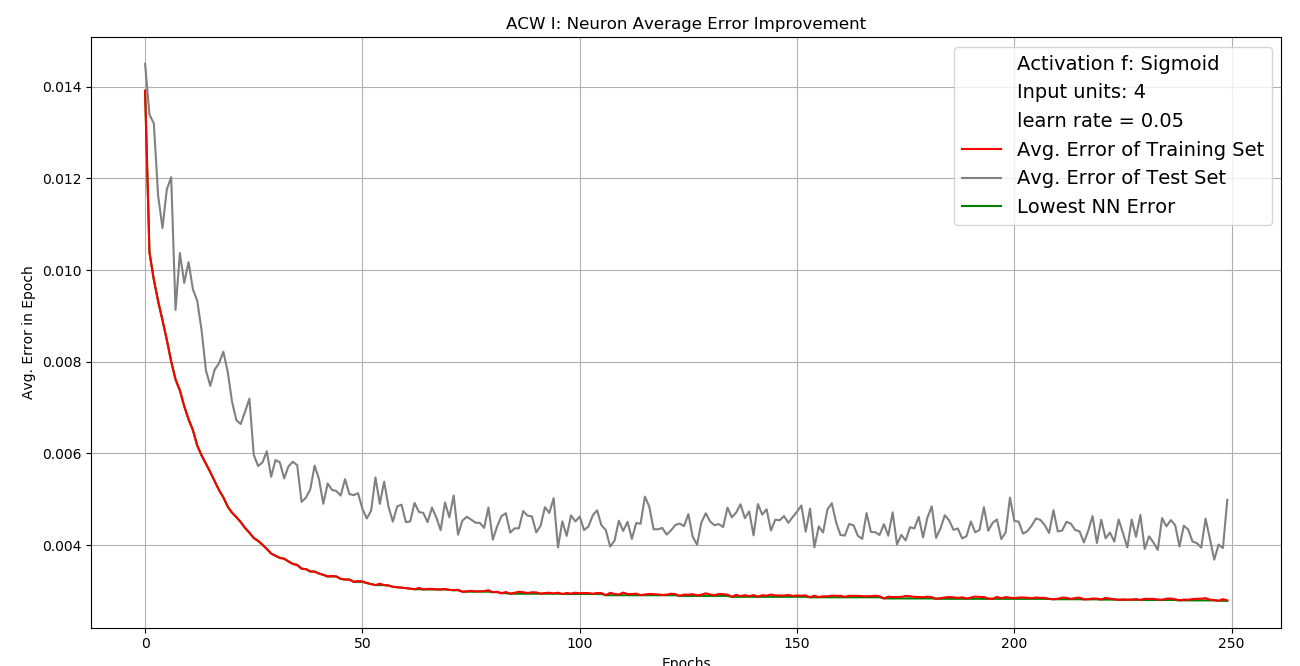
\includegraphics[width=0.65\textwidth]{my_images/acw_p1/task4_cross_learn_curve_without_shuffle.png}} & 
		\begin{tabular}[t]{@{}c@{}}
			
			\raisebox{-\height}{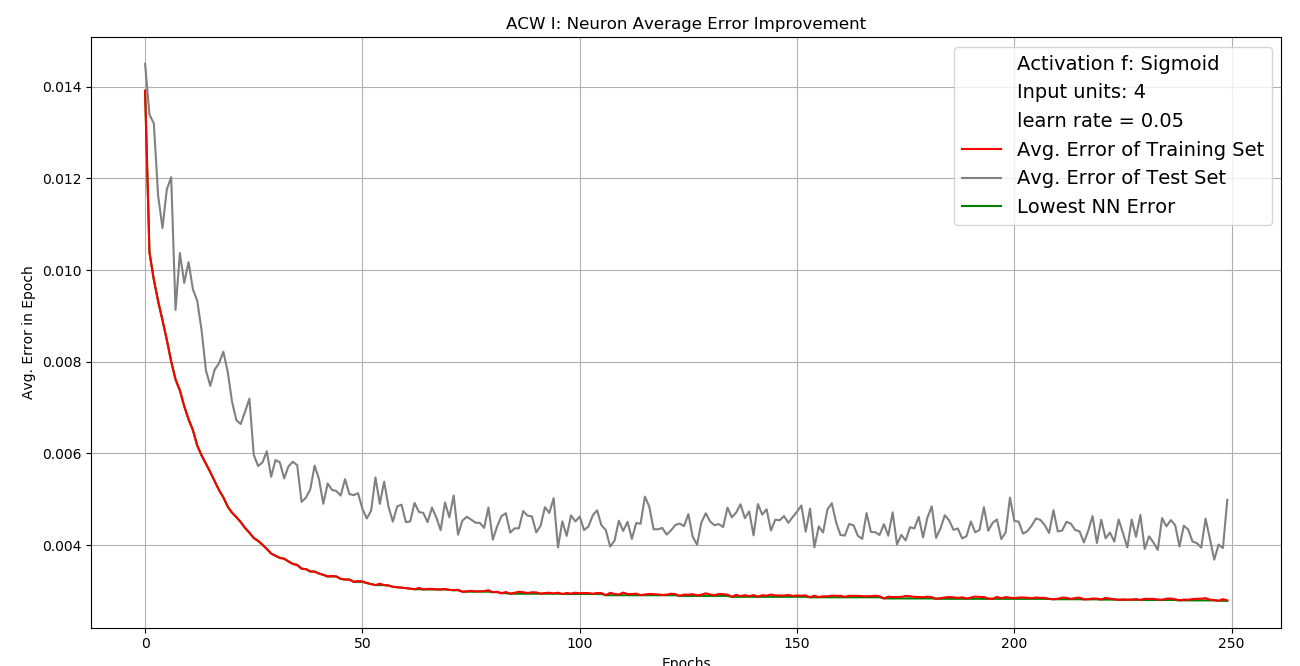
\includegraphics[width=0.3\textwidth]{my_images/acw_p1/task4_cross_learn_curve_without_shuffle.png}} \\
			\raisebox{-\height}{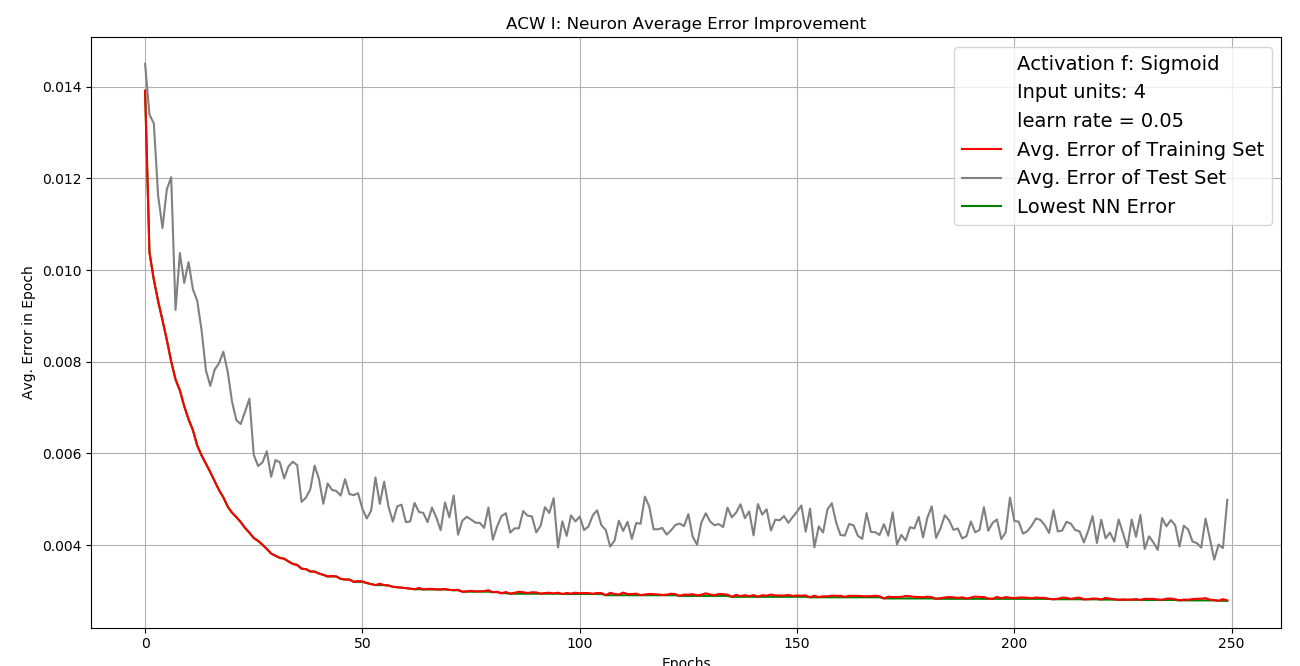
\includegraphics[width=0.3\textwidth]{my_images/acw_p1/task4_cross_learn_curve_without_shuffle.png}} \\
			
		\end{tabular}
	\end{tabular}
\end{figure}

\end{document}

